\section{Online Computation}
Offline computation is carried out once and the dependency files are saved. Every time the video is played, the online computation computes a selective mask for each frame and decodes according to the mask.

\subsection{Dependency File Accessing}
The standard file I/O is slow for random access in a large file because of the seeking overhead. The online computation utilizes the memory mapped I/O for fast random access of dependency files. 
%An example is given in the figure below,
%\begin{figure}
%\centering
%\vspace{2.5cm}
%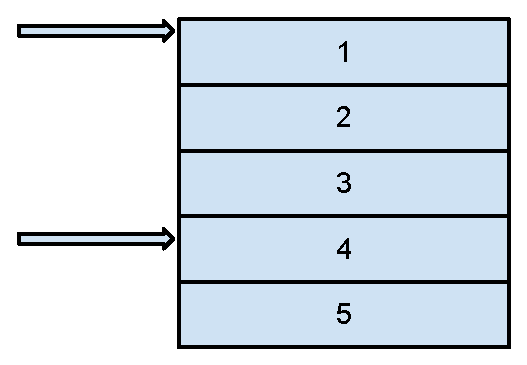
\includegraphics[height=1.7cm]{mmap.eps}
%\caption{Memory Mapped I/O for Dependency File Access}
%\end{figure}
Before accessing the content, the dependency file is mapped to memory using Linux mmap system call [webmmap] and a pointer to the first record is returned. Memory mapped I/O requires that each record occupies the same number of bytes. Suppose each record is 4 bytes and we need to access the sixth record, the pointer is moved by (6-1)*4=20 bytes. This approach facilities the fast random access of dependency file, with the price of padding the shorter records so that they can be aligned. 

\subsection{Selective Mask Computation}
Selective mask indicates the macroblocks that the decoder needs to decode as '1' and the rest as '0'. It considers both inter-VOP and intr-VOP dependencies. Note that the inter-VOP dependency has to be computed first. 
If intra-VOP dependency is computed first, when computing inter-VOP dependency, the computation will select some new P-macroblocks and I-macroblocks. Since the intra-VOP dependency for the newly selected I-macroblocks is not computed, this leads to decoding errors at those I-macroblocks. The error will subsequently affect the motion compensation decoding at other macroblocks using those I-macroblocks as reference. By contrast, if inter-VOP dependency is computed first, the intra-VOP computation will select only I-macroblocks because DC\&AC prediction coding only applies to I-macroblock. Since inter-VOP dependency does not apply to I-macroblocks, the newly selected I-macroblocks won't introduce errors. 

\subsubsection{Inter-VOP Dependency Computation}
Inter-VOP dependency is caused by motion compensation decoding. For a MPEG4 SP GOP, every I VOP is followed by a sequence of P VOPs.
%\begin{figure}
%\vspace{2.5cm}
%\centering
%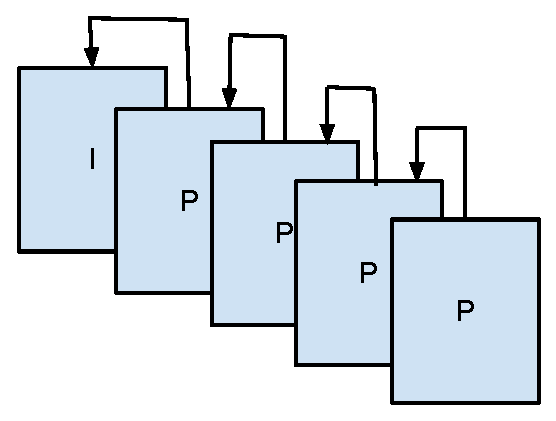
\includegraphics[height=1.8cm]{gop.eps}
%\caption{A GOP at MPEG4 Part2 SP}
%\end{figure} 
In a GOP, the P-macroblocks of every P frame are motion compensated with reference to macroblocks of its previous frame. This means every P frame is dependent on its previous frame and subsequently the dependency is one direction within a GOP. Based on this observation, we compute the inter-VOP dependency from last frame back to the first frame of the GOP. 

The dependencies are shown Fig 6(a). 
\begin{figure}
%\vspace{2.5cm}
\centering
%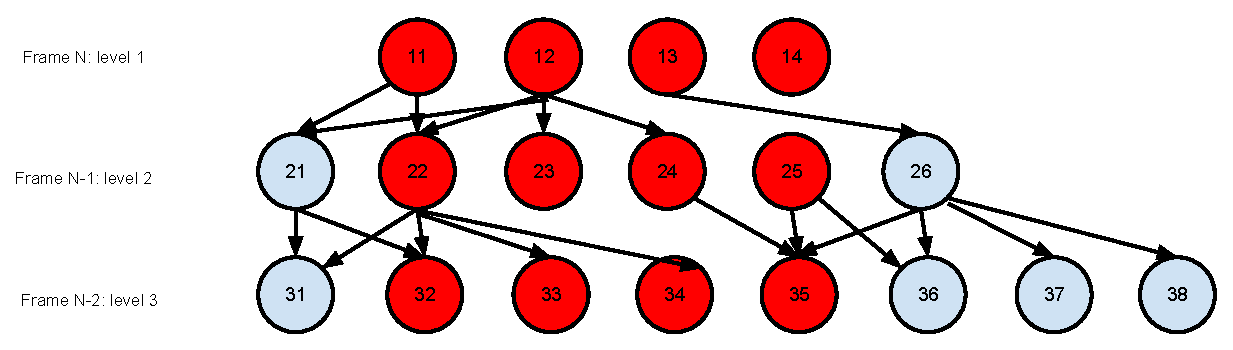
\includegraphics[height=2.5cm]{inter.eps}
\subfigure[Inter-VOP Graph]{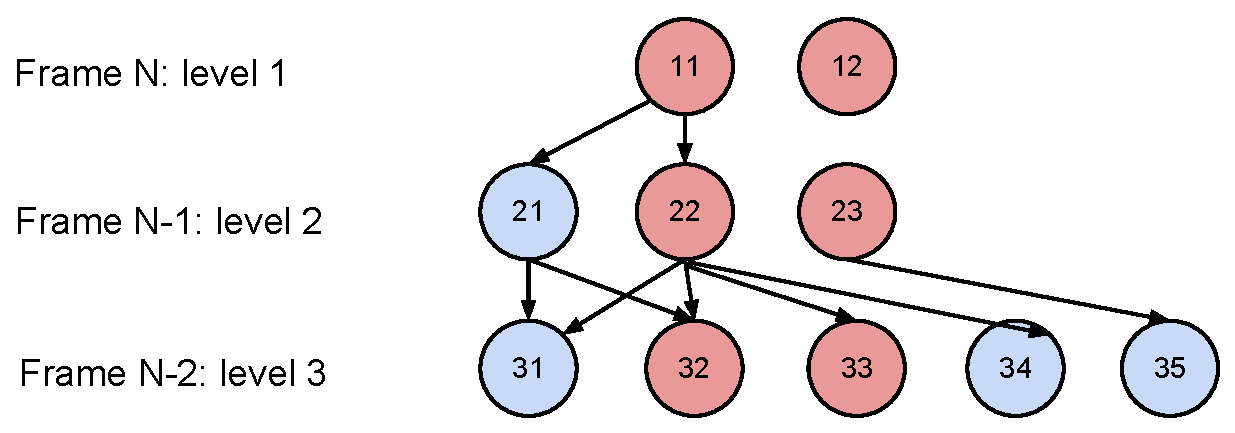
\includegraphics[height=1.8cm]{interc1.eps}}
\quad\quad
\subfigure[Modified Inter-VOP Graph]{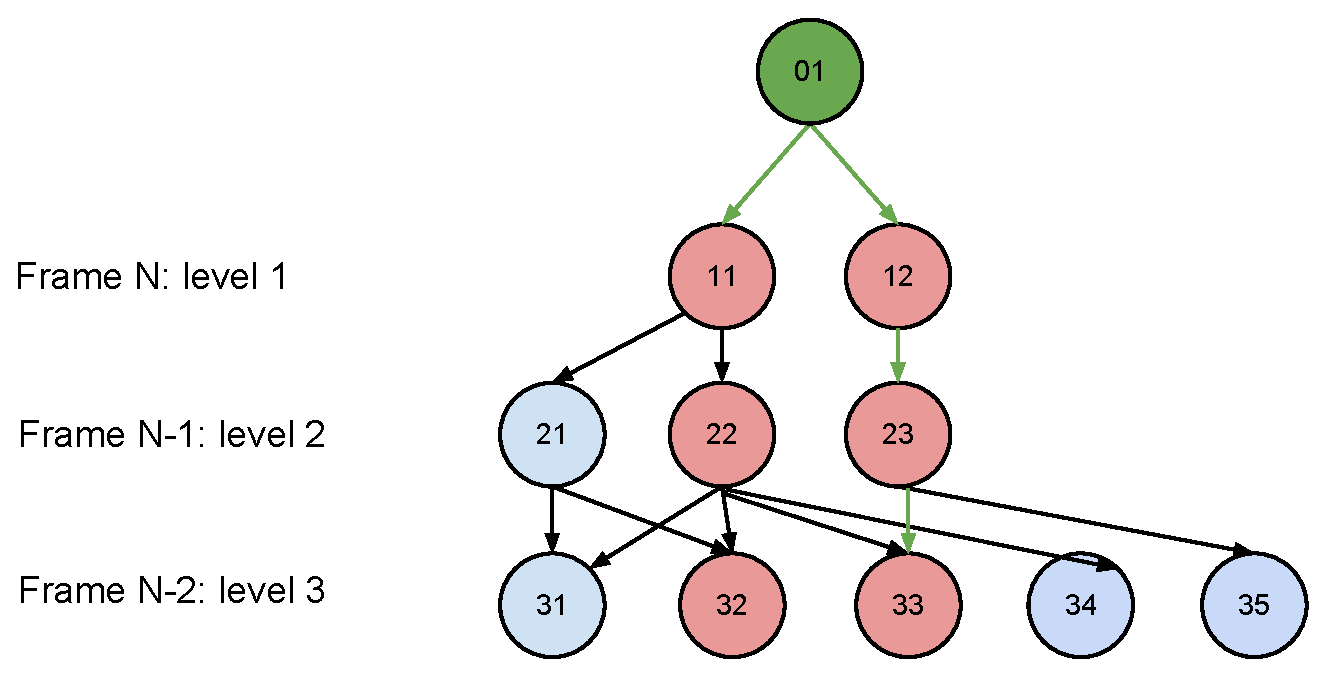
\includegraphics[height=2.7cm]{interc2.eps}}
\caption{Inter-VOP Dependency Abstraction} 
\end{figure}
Suppose frame N is the last frame of the GOP, the figure shows the dependency relationships among macroblocks in three VOPs. The macroblocks and the dependencies form a graph. With slight modification of adding a pseudo root node and edges connecting the ROI macroblocks, the graph is transformed to a weakly connected directed acyclic graph shown as Fig 6(b). 

%\begin{figure}
%\vspace{2.5cm}
%\centering
%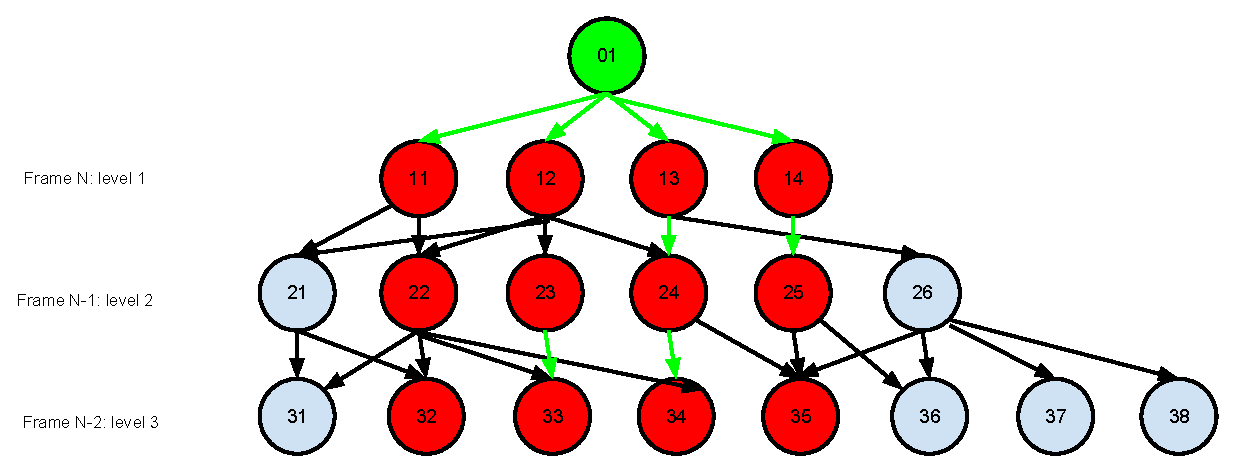
\includegraphics[height=2.5cm]{inter2.eps}
%\caption{Modified Inter-VOP Dependency Abstraction}
%\end{figure}

With this modification, the graph traversal algorithm Depth-First Traversal (DFT) or Breadth-First Traversal (BFT) can be applied. The macroblocks that are visited by the graph traversal are selected, while the rest are not needed. 

\subsubsection{Intra-VOP Dependency Computation} 
Simiar to Inter-VOP dependency, Intra-VOP dependency computation can be abstracted to graph traversal problems. 
\begin{figure}
%\vspace{2.5cm}
\centering
\subfigure[Graph]{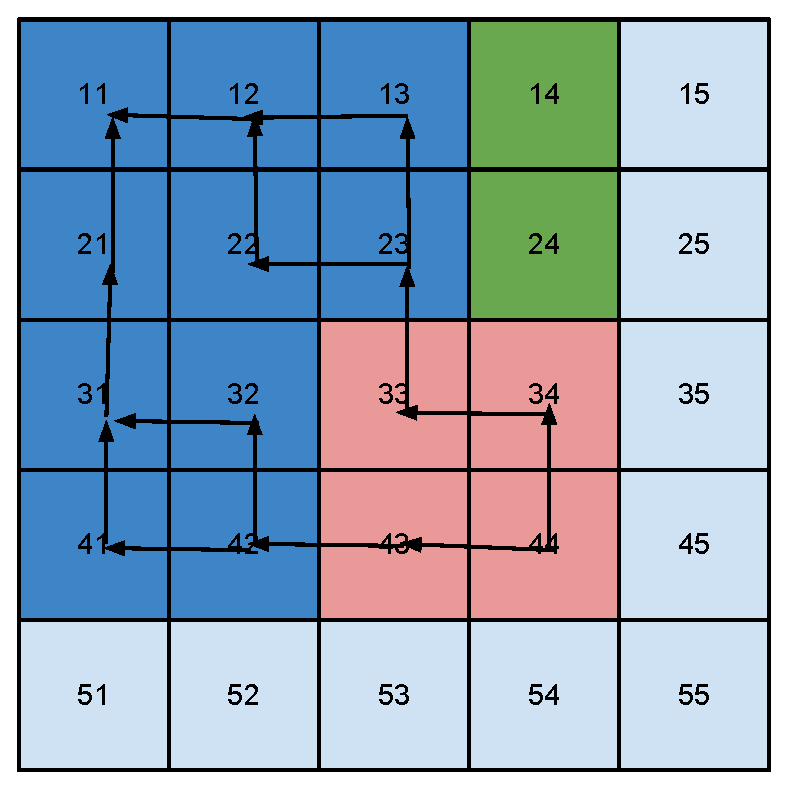
\includegraphics[height=2.5cm]{intrac1.eps}}
\quad\quad\quad
\subfigure[Optimization]{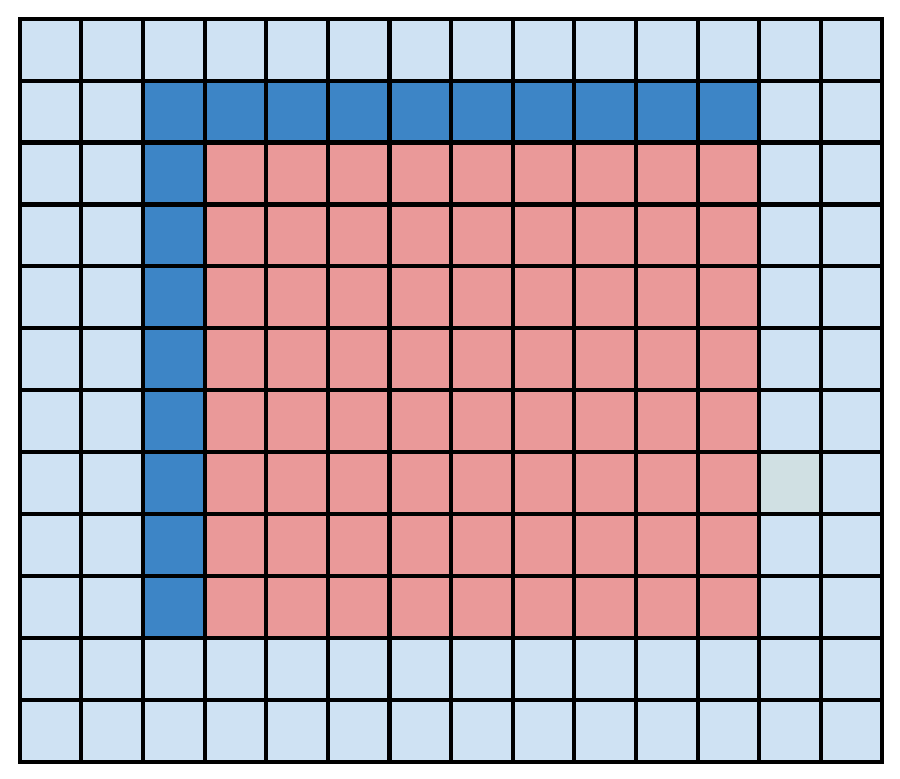
\includegraphics[height=2.5cm]{intrac2.eps}}
%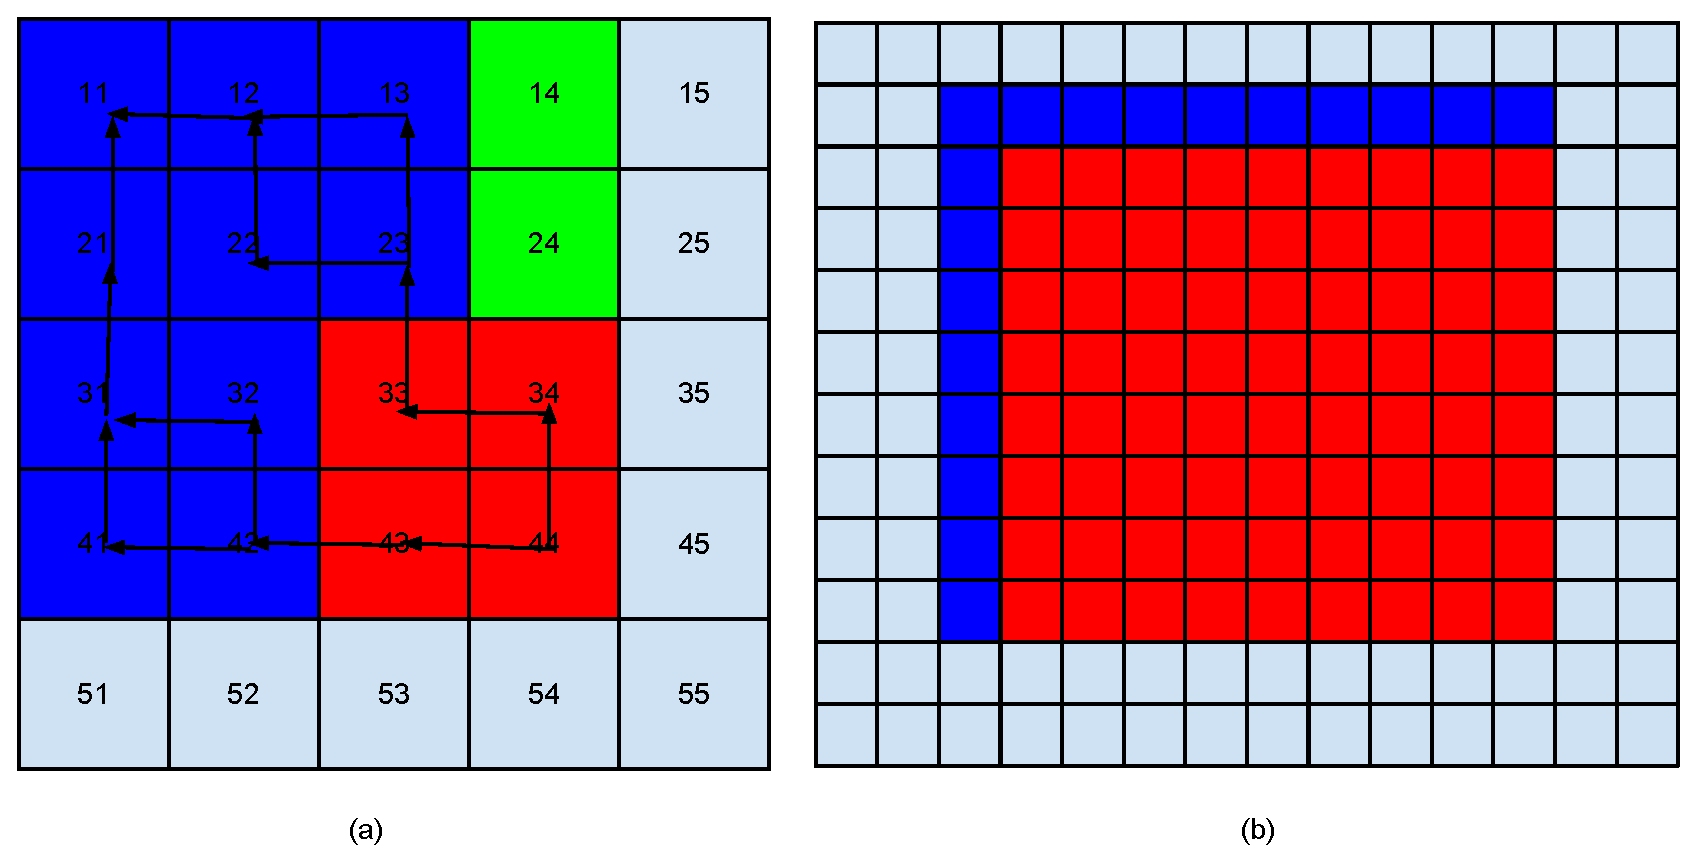
\includegraphics[height=2.5cm]{intra.eps}
\caption[intra.eps]{Intra-VOP Dependency and the Optimization}
\end{figure}
In Fig 7(a), suppose macroblock 33, 34, 43 and 44 are ROI macroblocks. The dependency graphs due to DC\&AC prediction coding is depicted. Because the dependency direction is always towarding up or left, the graph rooted at a macroblock is always formed by one of the graphs rooted at the first row and first column macroblocks of the ROI and some macroblocks within the ROI. Therefore, an optimization is to apply graph traversal algorithms only on the macroblocks at upper and left edges of the ROI, and select all macroblocks within ROI.

\subsubsection{Select the Bits}
The standard MPEG4 SP decoder is modified to decode selectively according to the selective mask. Because the decoder does not decodes all the bits, a mechanism is needed for the decoder to select the bits for selected macroblocks. 

Two approaches can be used to select the bits, which are depicted in figures below.
\begin{figure}
%\vspace{2.5cm}
\centering
%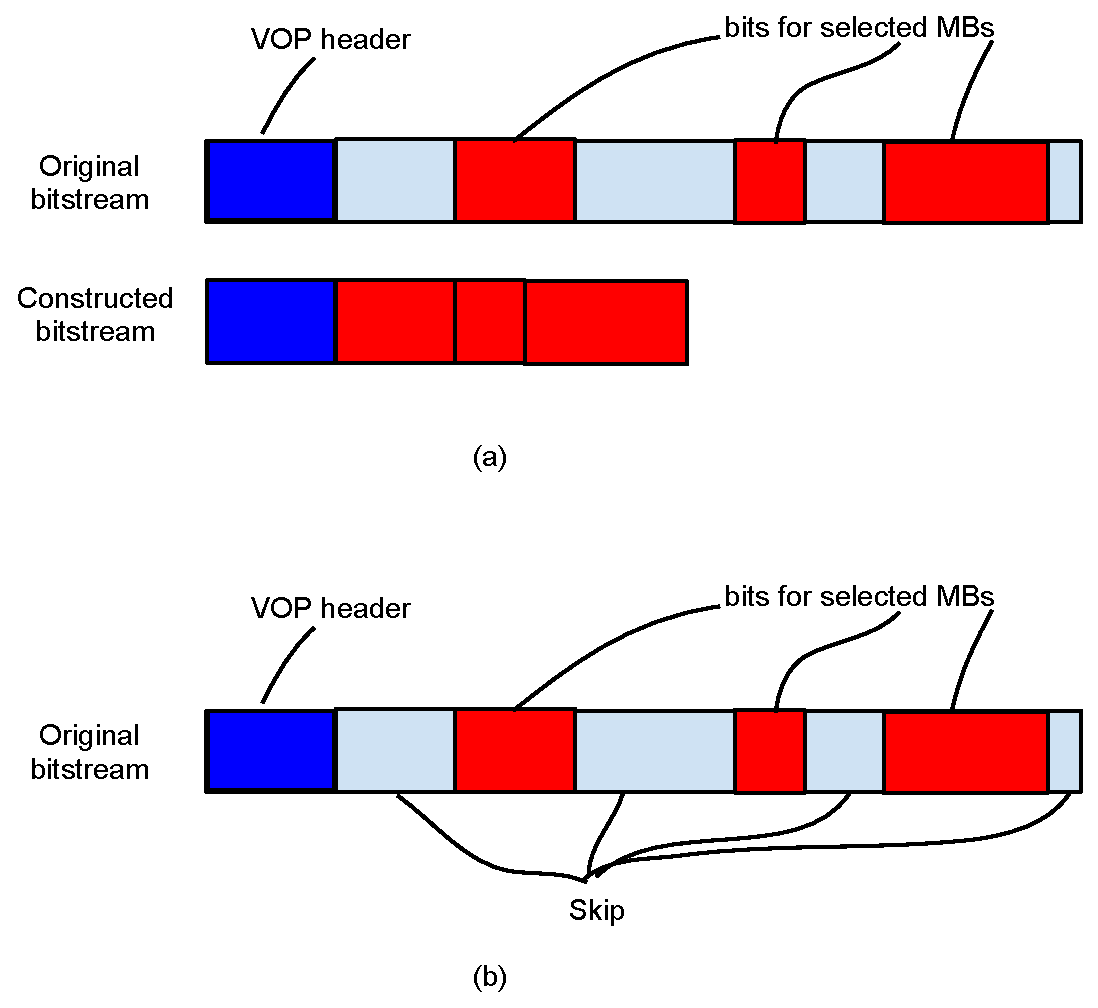
\includegraphics[height=2.5cm]{bits.eps}
\subfigure[Reconstruction]{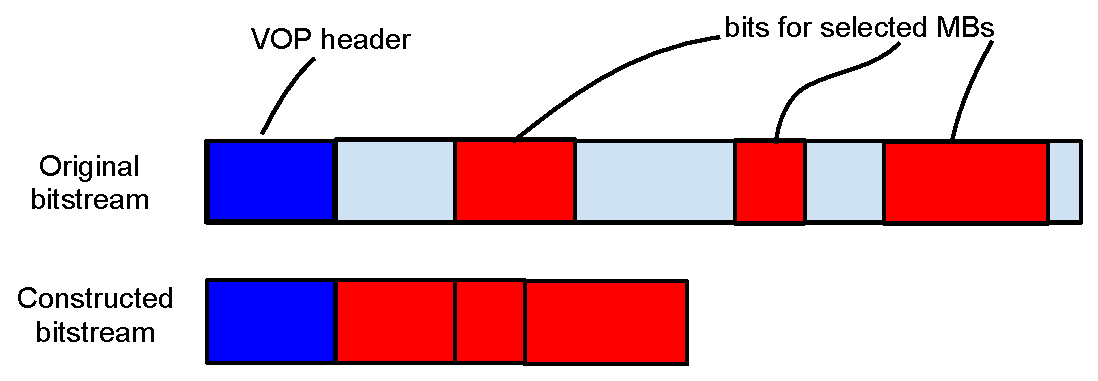
\includegraphics[width=5.6cm]{bits1.eps}}
\quad
\subfigure[Skip]{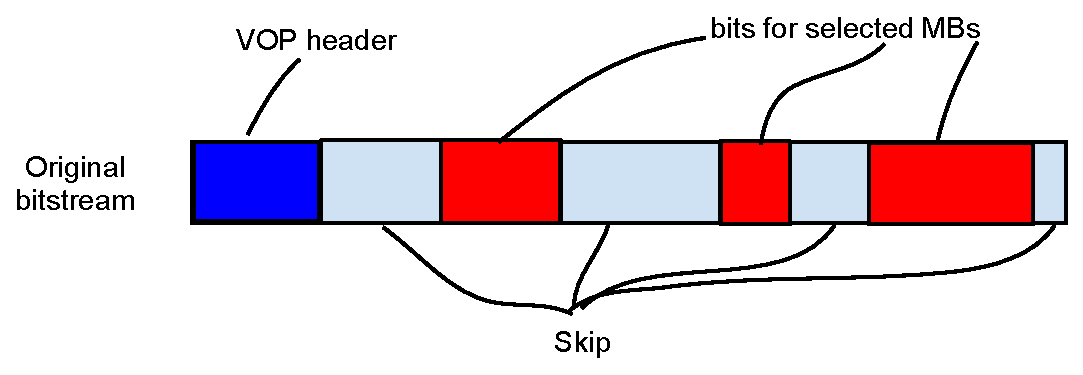
\includegraphics[width=5.6cm]{bits2.eps}}
\caption{Two different Approches of Selecting the Bits}
\end{figure}
Fig 8(a) illustrates the bitstream reconstruction approach, where a new video bitstream is constructed according to the selective masks and the macroblock start and end positions. Thew newly constructed bitstream consists of only the macroblocks selected in selective masks. The second approach is to instruct the decoder to seek to the start position of next selected macroblock at decoding, which is shown in Fig 8(b). The second approach avoids the additional memory allocation for the new bistream therefore it is the preferred approach in this project. However, for applications in the next streaming context, the first approach may provide some benefits in terms of bandwidth as the shorter reconstructed bitstream can be transmitted. 
\subsection{Modifications of Decoder}
The online computation requires modification for both motion decoding and texture decoding of standard MPEG4 SP decoder. For motion decoding, the MV values are loaded directly from MV dependency file. No MV prediction decoding is carried out. For texture decoding, the DC\&AC prediction direction is read from DC\&AC prediction direction file. The capability of bits seeking is also added for the decoder to decode selectively. 
  

